%!TEX root = ../thesis.tex
\chapter{Summary and Future Work}
\dblspace

Summary is just listing what you've done, one or 2 pages, then 'what we have found is that constrcution is possible, we can avoid the banana problem, limitations etc.

  Two salient routes of enquiry stem from where this work concludes: the continued accurate characterisation of 3D microstructure through histology, and the quantification of variability across animals; and the study into the functional consequences of incorporating microstructural detail into models, by simulating propagation and arrhythmias on geometries derived from both the newly available data and traditional methods and modalities.
  
  There is a wealth of histological data available today of the same and even higher quality and resolution than that which has been presented in this thesis. Many of these datasets have with them associated MRI and DTMRI images. A comprehensive characterisation of microstructure across many samples would, in and of itself, provide unprecedented anecdotal anatomical insight. But further, a comparison of the data across a range of samples allows a rigorous quantification of anatomical variability and the construction of 3D statistical tissue maps. Given the time consuming and inherently destructive nature of the histological process, there are a great many MRI and DTMRI datasets with no matching histology. The precise comparison of corresponding geometries obtained through DTMRI and of histological volumes, in particular in regions of heterogeneity such as rapidly varying fibre direction, papillary insertions, and tissue boundaries, could inform the interpretation of DTMRI in these uncertain zones in cases where no histology is available. For histological data paired with in vivo MRI, a final non-rigid volumetric registration of the coherent histology to the MRI could correct for distortions introduced by the experimental process, such as fixing, dehydration and unrepresentative pressure fields. This would provide volumes exquisitely accurate at every scale, from the entire organ down to the individual myocardial sheet.
  
 \begin{figure}[htbp]
   \centering
   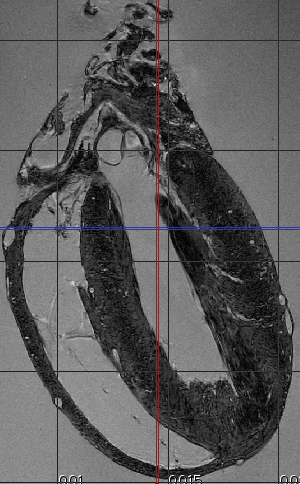
\includegraphics[width=0.45\textwidth]{Ch8/Figs/MRI}
   \caption{A tilted coronal cross-section of an MRI volume obtained from a rat heart in the same data set as the histology in Chapters 6 and 7.}
   \label{fig:MRI}
 \end{figure}
 
  The second line of investigation would aim to quantify the functional consequences of incorporating this detail into models. The wider hypothesis, that the inclusion of detail in highly heterogeneous zones promotes wave curvature and breakup and fosters arrhythmia, might be broken down into the following proposals.
  \begin{itemize}
    \item Sharp discontinuities are present at the papillary insertions and the junction of the septum with the myocardial free wall. Incoherent, crossing fibre directions are observed around the apex of the heart. It is proposed that rapidly varying fibre direction in these regions promotes wave curvature and helps to sustain arrhythmia.
    \item In the region of epicardial arteries, the anchoring effect is mitigated by the insulating tissue on the outside of epicardial arteries, when compared to simulations on the same geometries modelled solely as myocardium.
    \item The non-conducting interstitial spaces that divide the myocardium into sheets engender orthotropic conductivity on a macroscopic scale.
  \end{itemize}
  
  The hypotheses would be examined by simulating propagation and arrhythmias on geometries derived from several modalities, in regions where they differ significantly. Specifically, plane wave propagation and triggered arrhythmias will be simulated over the papillary muscle insertion, the apex, epicardial arteries and the junction of the septum and the free wall. In terms of fibre direction, four types of model could be used: those based solely on histology; those based on registered and segmented DTMRI; those with histological segmented geometry, but with DTMRI-derived fibre orientations; and those with DTMRI geometries and rule-based fibre orientations. The orthotropic effects of explicit sheet structure can be quantified, when compared to a reduced rate of diffusion across sheets from DTMRI, through the judicious design of stimulation protocols and simulation regimes. Single stimulation protocols can elucidate the effect of microstructure on wavefront curvature during normal cardiac function. Double stimulation protocols will initiate arrhythmia in ROIs, and times until cessation will be compared between the various substrate models. The lifetimes of reentrant waves, the numbers and interactions of singularity filaments, and the anchoring effect of heterogeneities on filaments would be analysed. Subject to the availability of data, it would be possible to study the effects of pathological remodelling on function with these techniques, for example, in cases of infarct or hypertrophic cardiomyopathy.
  
  Finally, spatiotemporal data from 4D in vivo MRI permits the investigation of mechanical function and dysfunction and its relationship to microstructure. Active contractile simulations of cardiac electromechanics, based on accurate tissue type, sheet structure and fibre direction from histology, can be parameterised and validated by their mapping to measured contraction paths.
